\section{Performance}
\label{sec:expts}

This section quantifies the computational cost of $\Pi_\bin$, our protocol for computing verifiable DP counting queries. 
All results reported below were run on a \textit{single} core of an Apple M1 Mac and the code to reproduce these results can be found at \url{https://github.com/abiswas3/Verifiable-Differential-Privacy}.\par
%When the prover is trusted to perform aggregations correctly, the binomial mechanism  simply involves summing over $n$ inputs, sampling one draw of Binomial noise and aggregating the results.
%Meanwhile, in our protocol, the verifier must check if the included client inputs are legal. 
%Then it must verify that the prover sampled noise from the correct distribution along with performing aggregation correctly. 
% In Table \ref{tab:pipeline} we describe the latency of the different phases of $\Pi_\bin$. 
In all our experiments, we instantiate the homomorphic commitment scheme using Pedersen Commitments (PC) \cite{pedersen1991non} over the Ristretto curve\footnote{\url{https://doc.dalek.rs/curve25519_dalek/ristretto/struct.RistrettoPoint.html}}. 
A single commitment operation requires two multiplications and one addition and takes 156 $\mu s$. 
We instantiate $\oracle_{\texttt{Morra}}$ using $\Pi_{\texttt{Morra}}$ described in Section \ref{sec: commitments}.
We instantiate $\oracle_{\texttt{OR}}$ with the non-interactive Fiat-Shamir transform of the $\Sigma$-OR protocol described in Appendix \ref{app:sigma_open} using SHA-3\footnote{\url{https://docs.rs/sha3/latest/sha3/}} as the random oracle. 
In the experiments discussed below, each client $i \in [n]$ sends commitments to their inputs and a non-interactive $\Sigma$-OR proof of their 
validity.
Additionally, each client sends the prover(s) openings to its commitments as described in Line 2 of Figure \ref{fig:dp_interactive_proof}. \par
Table \ref{tab:pipeline} describes the latency of different stages $\Pi_\bin$ with parameters $n=10^6, \epsilon=0.095, \delta= 10^{-10} $, in relation to Figure \ref{fig:dp_interactive_proof}. Note that for the fixed value of $\delta=10^{-10}$, $\epsilon=0.095$ corresponds to $\noisen=262144$.

\begin{enumerate}
    \item{The first column C-Verify describes the time it takes for the verifier to validate $n=10^6$ client $\Sigma$-OR proofs sequentially (Lines 3-4).}

    \item{The second column Bit-commit describes the time it takes a single prover to sample $\noisen$ private bits and create $\noisen$ non-interactive $\Sigma$-OR proofs of their validity (Lines 5-6).}

    \item{The third column P-Verify, describes how long it takes the verifier to validate these proofs (Line 7).}

    \item{The fourth column describes the time it takes to play Morra, i.e., commit, open and aggregate $\noisen$ values in $\Z_q$ (Lines 9-10).}

    \item{The fifth column describes the time it takes to aggregate $\noisen + n$ vales in $\Z_q$ (Line 11).}

    \item{Finally the last column describes the time it takes to check the provers outputs are correct (Lines 12-13).}
\end{enumerate}

We remark that numbers reported in the table result from running computations sequentially on a single core. 
As each round of $\Pi_\bin$ is independent of the other rounds, these computations could also be run in parallel. 
As our main bottleneck is working with the $\Sigma$-proof creation and verification, Figure~\ref{fig:esp_vs_coins} describes how proof creation and verification latency scales with the privacy parameter $\epsilon$ (or number of private coins $\noisen$). Note that for high privacy settings (small values of $\epsilon$), the prover(s) need to generate more private coins to ensure indistinguishability. Specifically, the number of coins ($n_b$) is proportional to $1/\epsilon^2$ (Lemma~\ref{theorem:dp_guarantee}), and the time cost is then linear in $n_b$. 


 
 \begin{table}[]
 \caption{The table below benchmarks the latency of each stage of $\Pi_\bin$ for computing single dimension counting queries with parameters $n=10^6, \epsilon=0.095, \delta= 10^{-10} $.  For a fixed value of $\delta$, an $\epsilon=0.095$ corresponds to $\noisen=262144$ private coins for the binomial mechanism.}
\label{tab:pipeline}
\begin{tabular}{|l|l|l|l|l|l|l|}
\hline
C-Verifiy & Bit-commit & P-Verify & Morra & Agg  & Check     \\ \hline
169 sec & 53 sec        & 45 sec   & 33 sec & 79 ms  & 189 ms \\ \hline
\end{tabular}
\end{table}

 \begin{figure}[t]
     \centering    
     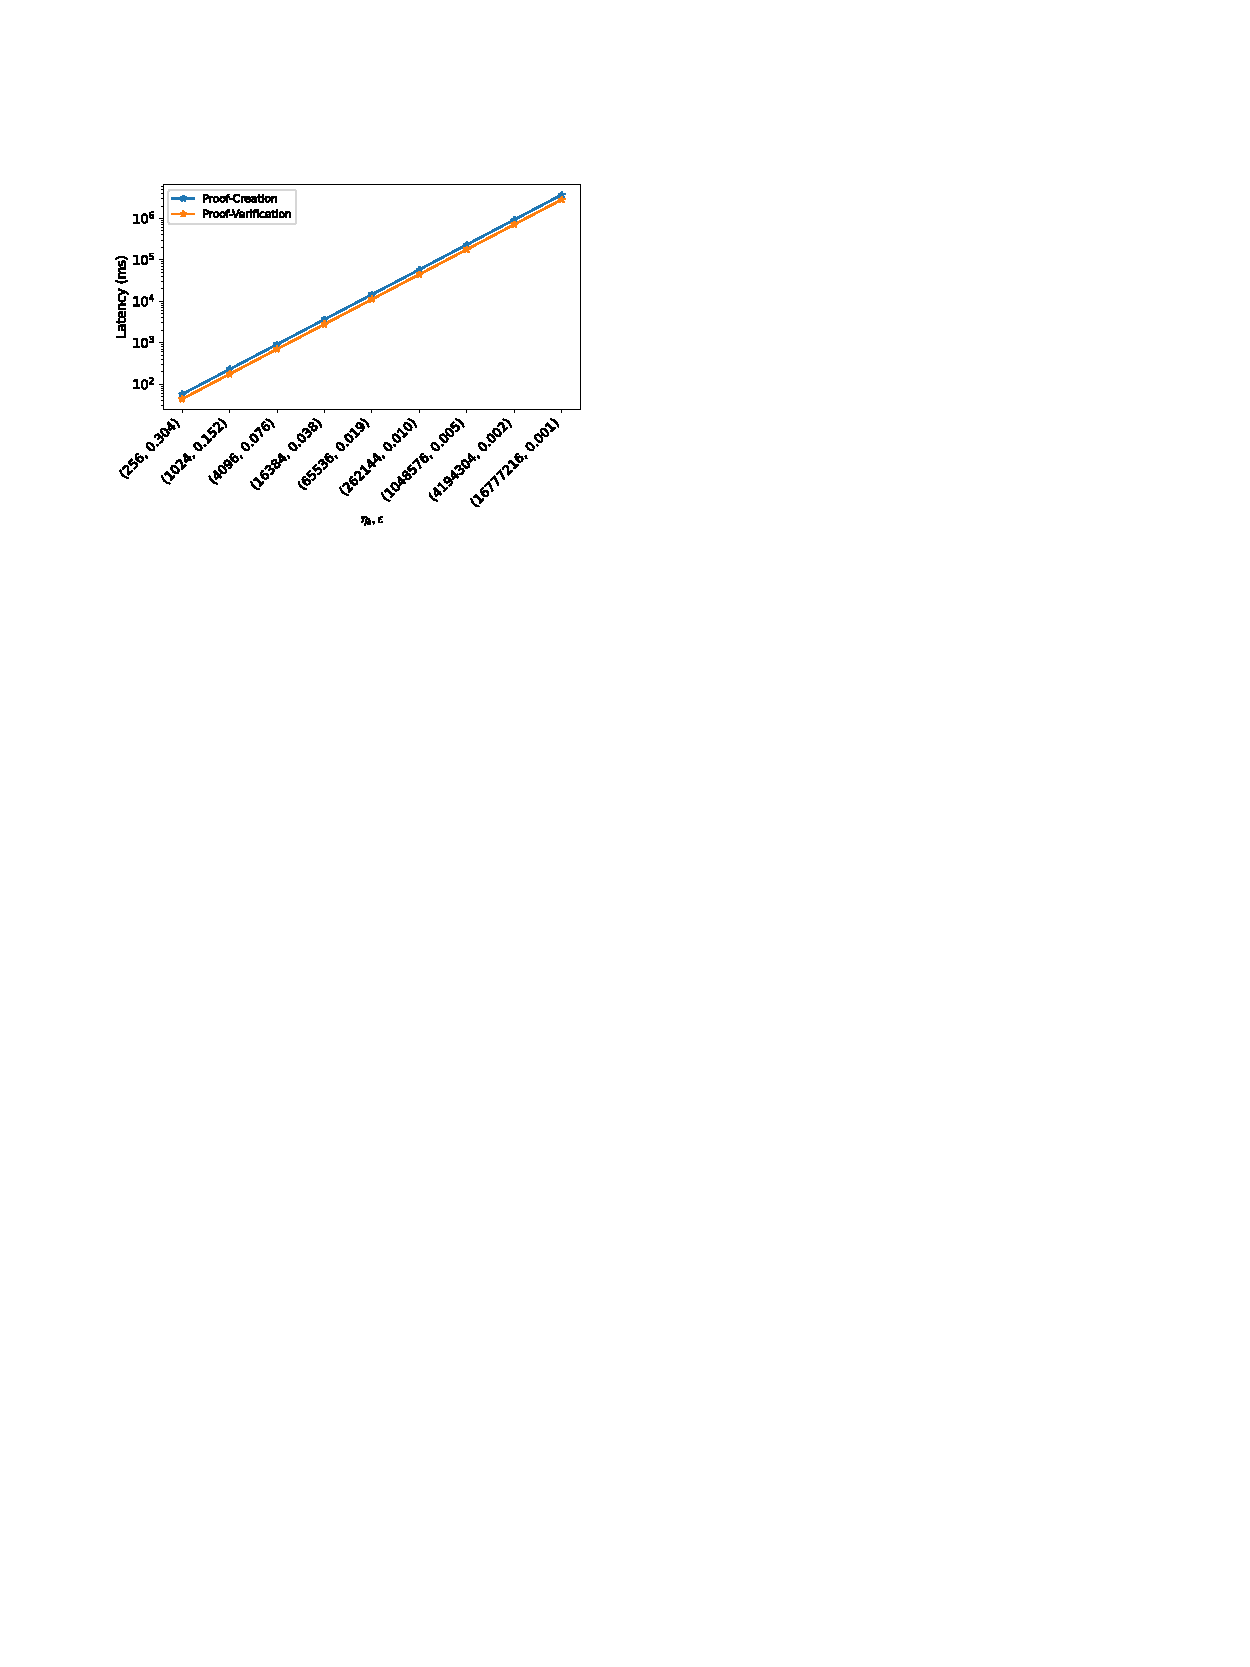
\includegraphics[scale=0.85]{pngs/eps_vs_coins.pdf}
     \caption{The figure above describes the latency of $\Sigma$-proof creation and verification as a function of the privacy parameters $\noisen$ and $\epsilon$. For a fixed $\delta=10^{-10}$, $\epsilon$ and $\noisen$ have one to one correspondence given by Lemma $\ref{theorem:dp_guarantee}$.}
     \label{fig:esp_vs_coins}
 \end{figure}


\paragraph{Time cost for client verification (MPC case)}
Clients submit secret shares of their inputs in the MPC setting. Thus the servers must verify that the client inputs are valid. For $M$-dimensional DP-histogram estimation, the client inputs are restricted to one-hot encoded vectors of size $M$. As discussed in Section \ref{sec:client_verification}, the sketching techniques used in PRIO and Poplar allow servers to verify clients with information-theoretic security. Still, they are vulnerable to attacks by malicious servers. Our use of $\Sigma$-OR-protocols can defend against such attacks, but it comes at a higher computational cost due to its reliance on commitments (which assume one-way functions exist). 
Figure~\ref{fig:client_verification} benchmarks the increase in latency as a function of the number of dimensions ($M$) of client input. We remark that the numbers in Figure \ref{fig:client_verification} are pessimistic as the Sigma-OR proof can be parallelised across the $M$ dimensions (at the cost of communication complexity), whereas the sketching techniques cannot as they are based on the inner products.
 \begin{figure}[t]
     \centering    
     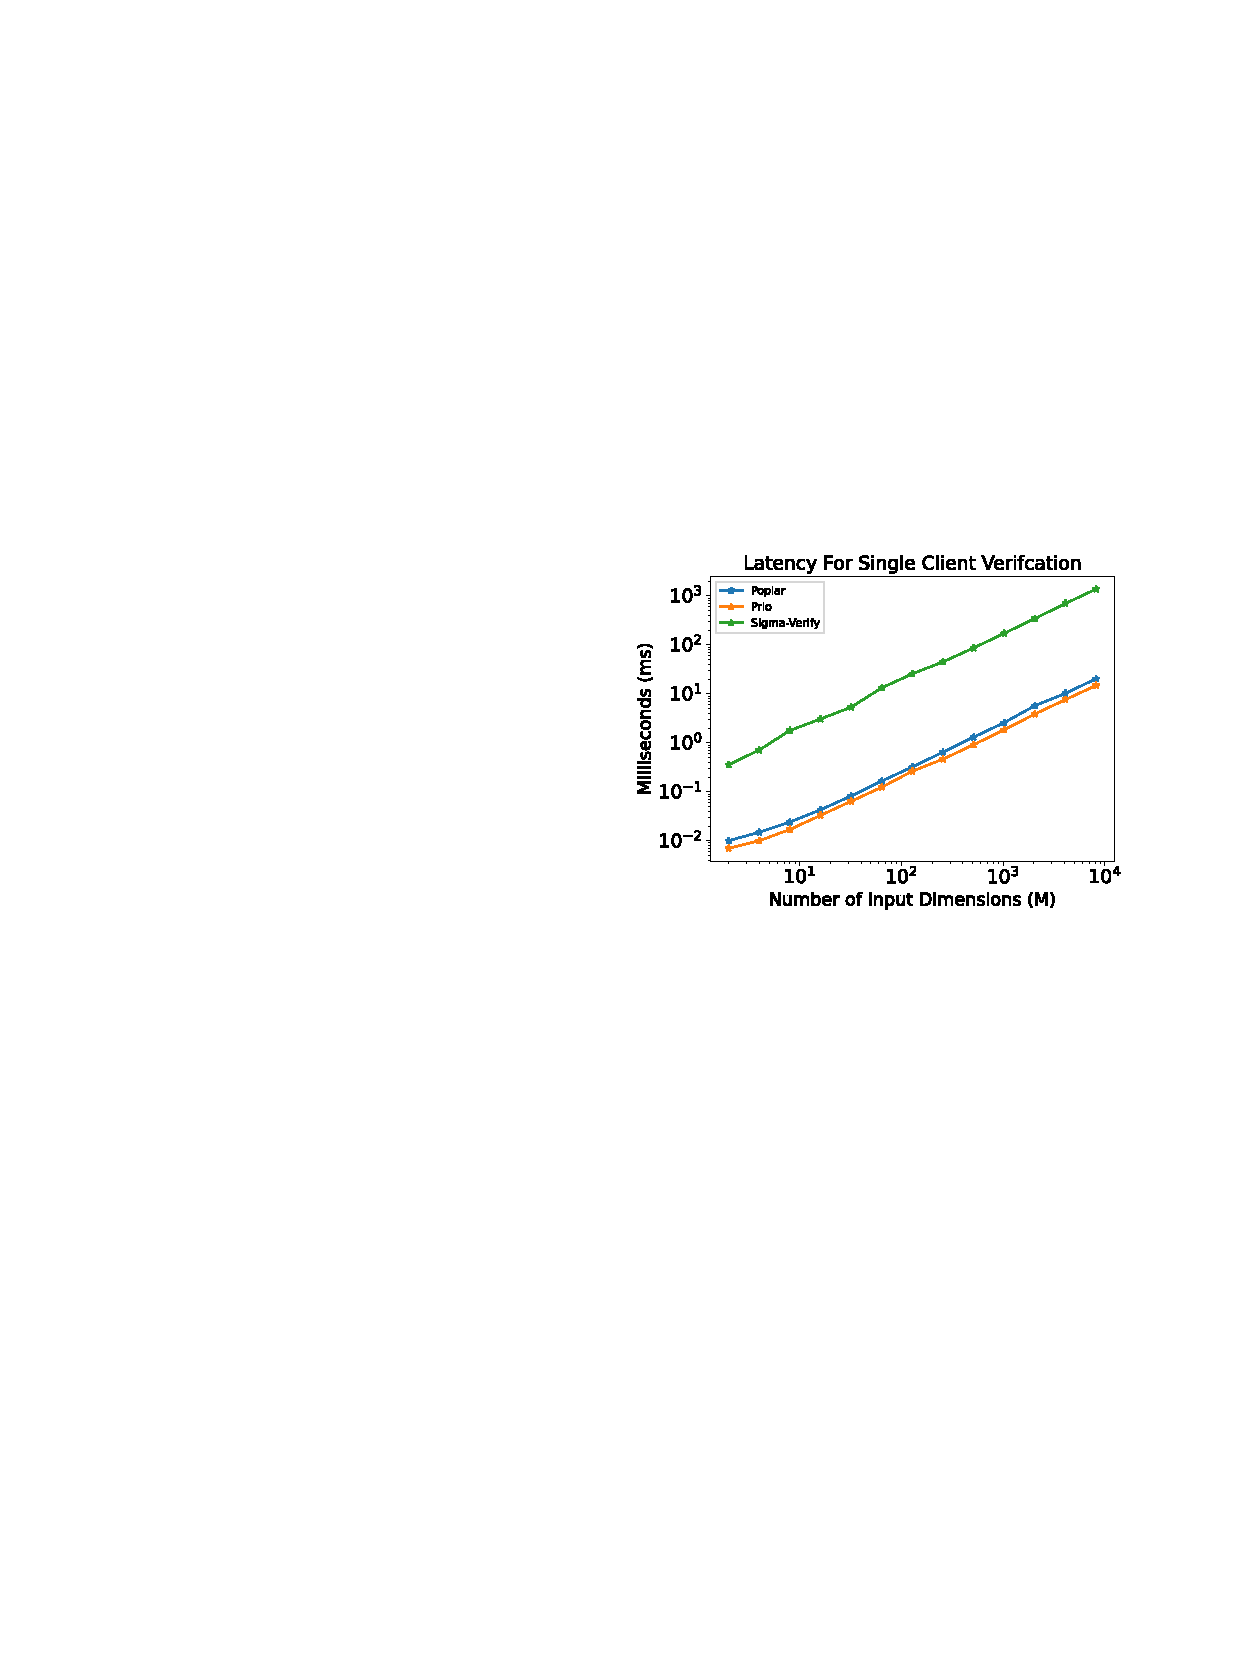
\includegraphics[scale=0.9]{pngs/verification_times.pdf}
     \caption{The figure above describes the performance cost for using a Sigma protocol to verify that the client's commitment is wellformed. PRIO and Poplar use lightweight sketching protocols and general-purpose MPC to check in zero knowledge whether a client's input is a one-hot vector and do not need to assume one-way functions exist. But as described earlier, they are susceptible to collusion attacks.}
     \label{fig:client_verification}
 \end{figure}

